\documentclass{article}

\usepackage{arxiv}

\usepackage[utf8]{inputenc} % allow utf-8 input
\usepackage[T1]{fontenc}    % use 8-bit T1 fonts
\usepackage{lmodern}        % https://github.com/rstudio/rticles/issues/343
\usepackage{hyperref}       % hyperlinks
\usepackage{url}            % simple URL typesetting
\usepackage{booktabs}       % professional-quality tables
\usepackage{amsfonts}       % blackboard math symbols
\usepackage{nicefrac}       % compact symbols for 1/2, etc.
\usepackage{microtype}      % microtypography
\usepackage{graphicx}

\title{Transnational social connectedness and the 2016 Referendum on the
UK's Membership of the European Union}

\author{
    Owen Winter
   \\
    School of Geographical Sciences \\
    Bristol University \\
  Bristol BS8 1RL \\
  \texttt{\href{mailto:owen.winter.2021@bristol.ac.uk}{\nolinkurl{owen.winter.2021@bristol.ac.uk}}} \\
  }


% tightlist command for lists without linebreak
\providecommand{\tightlist}{%
  \setlength{\itemsep}{0pt}\setlength{\parskip}{0pt}}

% From pandoc table feature
\usepackage{longtable,booktabs,array}
\usepackage{calc} % for calculating minipage widths
% Correct order of tables after \paragraph or \subparagraph
\usepackage{etoolbox}
\makeatletter
\patchcmd\longtable{\par}{\if@noskipsec\mbox{}\fi\par}{}{}
\makeatother
% Allow footnotes in longtable head/foot
\IfFileExists{footnotehyper.sty}{\usepackage{footnotehyper}}{\usepackage{footnote}}
\makesavenoteenv{longtable}

% Pandoc citation processing
\newlength{\cslhangindent}
\setlength{\cslhangindent}{1.5em}
\newlength{\csllabelwidth}
\setlength{\csllabelwidth}{3em}
\newlength{\cslentryspacingunit} % times entry-spacing
\setlength{\cslentryspacingunit}{\parskip}
% for Pandoc 2.8 to 2.10.1
\newenvironment{cslreferences}%
  {}%
  {\par}
% For Pandoc 2.11+
\newenvironment{CSLReferences}[2] % #1 hanging-ident, #2 entry spacing
 {% don't indent paragraphs
  \setlength{\parindent}{0pt}
  % turn on hanging indent if param 1 is 1
  \ifodd #1
  \let\oldpar\par
  \def\par{\hangindent=\cslhangindent\oldpar}
  \fi
  % set entry spacing
  \setlength{\parskip}{#2\cslentryspacingunit}
 }%
 {}
\usepackage{calc}
\newcommand{\CSLBlock}[1]{#1\hfill\break}
\newcommand{\CSLLeftMargin}[1]{\parbox[t]{\csllabelwidth}{#1}}
\newcommand{\CSLRightInline}[1]{\parbox[t]{\linewidth - \csllabelwidth}{#1}\break}
\newcommand{\CSLIndent}[1]{\hspace{\cslhangindent}#1}

\begin{document}
\maketitle


\begin{abstract}

\end{abstract}

\keywords{
    EU Referendum
   \and
    Euroscepticism
   \and
    Facebook
   \and
    Migration
   \and
    Social Connectedness
   \and
    Social Media
   \and
    Voting
  }

\hypertarget{introduction}{%
\section{Introduction}\label{introduction}}

There is a broad literature on the social transmission of social and
political values (Huckfeldt and Sprague 1987; Lee et al. 2017;
Nurmuhammad et al. 2016) and the effect of social contact on perceptions
of out-groups (Enos 2017). In the digital age, the social connections
along which political views might be transmitted can be quantified more
easily. This study investigates the effect of transnational social
connectedness on voting patterns in the United Kingdom's 2016 Referenfum
on membership of the European Union, using Facebook's Social
Connectedness Index (SCI) (T. K. Bailey R. Cao and Wong. 2018).

The research question of this study is \textbf{Did transnational
Facebook connections with individuals in other EU member states reduce
the likelihood of voting to leave the EU?}

\hypertarget{hypotheses}{%
\section{Hypotheses}\label{hypotheses}}

Testable hypotheses are set up to elucidate the research question. These
hypotheses are based on theorised relationships between transnational
social connections, migration and EU referendum vote choice (Figure
\ref{fig:effects}). While the main purpose of this study is to consider
the effects of transnational social connections on EU referendum voting,
individual-level data on these connections is not available. This means
using aggregated data, which is closely related to other variables which
may affect voting patterns.

\begin{figure}
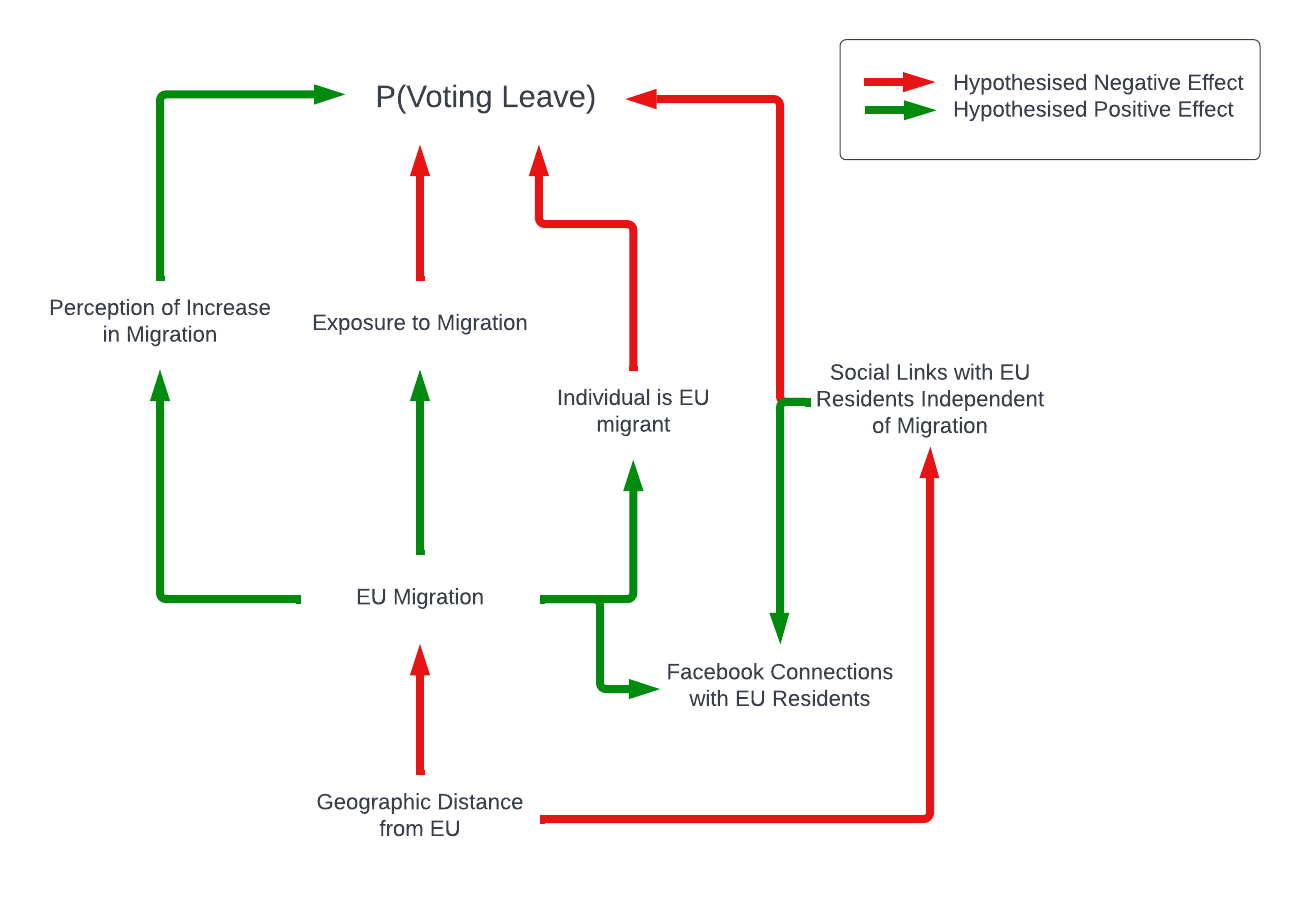
\includegraphics[width=1\linewidth]{images/Effects} \caption{Hypothesised Effects of Migration and Social Connectedness on EU Referendum Voting}\label{fig:effects}
\end{figure}

As illustrated in Figure \ref{fig:effects}, Facebook connections between
UK and EU residents are shaped by migration, because it is expected that
migrants have high levels of connectedness to origin countries
(\textbf{H1}).

~~~~~~~\textbf{H1: Areas with higher levels of EU migration tend to have
higher levels of social connectedness with EU residents}

The effects of migration on voting operate at both the individual level
and as a contextual effect. It is expected that EU migrants are less
likely to vote to leave the EU because of the risks to continued freedom
of movement. In line with Goodwin and Milazzo (2017), it is hypothesised
that the presence of EU migrants in an area had a negative effect on the
likelihood of voting to leave the EU, both through the individual-level
effect and because exposure to migrants reduces anti-migrant sentiment,
leading to more positive assessments of membership of the EU
(\textbf{H2}). Meanwhile, increases in the \emph{rate} of migration
locally had a positive effect on likelihood to vote to leave the EU,
because of a perception of undesirable change (\textbf{H3}).

~~~~~~~\textbf{H2: The presence of EU migrants in an area has a negative
effect on likelihood of voting to leave the EU}

~~~~~~~\textbf{H3: Recent increases in the volume of EU migration in an
area has a positive effect on likelihood of voting to leave the EU }

As a result of these migration-related effects, it is expected that
areas which voted to remain in the EU will have higher levels of social
connectedness with EU residents (\textbf{H4}). This is not necessarily a
causal relationship, but reflects the fact that areas with higher levels
of EU migration tended to vote to remain in the EU.

~~~~~~\textbf{H4: Areas which voted to remain in the EU tend to have
higher levels of social connectedness with EU residents}

Finally, the aim of this study is to isolate the effect of social
connectedness with EU residents independent from the individual and
contextual effects of migration discussed above. It is hypothesised that
social connections will have an independent negative effect on the
likelihood of voting to leave the EU, because of the social transmission
of positivity towards other EU nations and reduced negativity towards EU
migration (\textbf{H5}). This is consistent with the findings of M.
Bailey et al. (2020), that, across the EU, euroscepticism decreases with
the share of a region's Facebook connections that are to regions in a
different European country.

~~~~~~~\textbf{H5: Social connectedness with EU residents has a negative
effect on the likelihood of voting to leave the EU}

\hypertarget{data}{%
\section{Data}\label{data}}

\hypertarget{facebook-social-connectedness-index-sci}{%
\subsection{Facebook Social Connectedness Index
(SCI)}\label{facebook-social-connectedness-index-sci}}

The SCI is published by Facebook (T. K. Bailey R. Cao and Wong. 2018) to
study connections across geographic regions. It is produced by assigning
Facebook users to geographic areas using profile information, before
counting and scaling the number of connections between pairs of areas.
Areas with few friendships are dropped and random noise is added to
ensure anonymity. The SCI is the number of possible friendships between
two regions which are fulfilled, per billion.

\[Social Connectedness_{i,j} = \frac{FB\_Connections_{i,j}}{FB\_Users_{i}*FB\_Users_{j}}\]

The lowest level in the UK which SCI is measured at is GADM regions,
which are concurrent with NUTS regions (Global Administrative Areas
2022). Table \ref{table:loadSCI} shows the highest SCI scores including
UK regions. As one might expect, the highest scores are within-region,
with the highest proportion of friendships fulfilled within UKM66
(Shetland Islands).

\begin{longtable}[]{@{}llr@{}}
\caption{\label{table:loadSCI}Highest SCI scores at GADM-level, all
pairs including UK regions}\tabularnewline
\toprule
Region 1 & Region 2 & SCI \\
\midrule
\endfirsthead
\toprule
Region 1 & Region 2 & SCI \\
\midrule
\endhead
UKM66 & UKM66 & 61610896 \\
UKM65 & UKM65 & 52441781 \\
UKM64 & UKM64 & 39082660 \\
UKL11 & UKL11 & 15893326 \\
UKN16 & UKN16 & 12226389 \\
UKN10 & UKN10 & 11714844 \\
\bottomrule
\end{longtable}

To study the effect of transnational friendships, SCI scores must be
aggregated at higher-levels than GADM1 for regions outside the UK.
Because Facebook does not share this information, the closest
approximation is a population weighted average. This approach assumes
that \(Facebook\_Users_{i}\) in the equation above is approximately
proportional to the population of region \(i\). This is necessary to
produce coherent units for analysis. In the EU, GADM1 regions are
concurrent with NUTS regions, so NUTS population data can be used
(eurostat 2021).

\begin{longtable}[]{@{}llrr@{}}
\caption{\label{table:countrySCI}Highest SCI scores between UK regions
and other countries}\tabularnewline
\toprule
UK Region & Country & Mean SCI & Population Weighted Mean SCI \\
\midrule
\endfirsthead
\toprule
UK Region & Country & Mean SCI & Population Weighted Mean SCI \\
\midrule
\endhead
UKN11 & TLS & 106071 & 106071 \\
UKN10 & IE & 67299 & 50373 \\
UKN16 & IE & 56769 & 44639 \\
UKJ31 & VCT & 37680 & 37680 \\
UKE42 & TCA & 34643 & 34643 \\
UKI32 & MCO & 34200 & 34200 \\
\bottomrule
\end{longtable}

Table \ref{table:countrySCI} shows UK NUTS regions and their scaled SCI
with countries excluding the UK. The most connected regions are UKN11
(Mid Ulster) and TLS (East Timor). An article by The Belfast Telegraph
(Peake 2014) suggests that there is a genuine connection, however, the
presence of Timor-Leste also shows the limitations of the SCI. The SCI
measures the proportion of all possible connections fulfilled, rather
than the proportion of residents. In the East Timorese case, it may be
that a small minority of Mid Ulster residents have many East Timorese
connections, rather than a large proportion of those in Mid Ulster
having a connection to East Timor.

Principal components analysis (PCA) can be used for discriptive
analysis, showing some of the associations between UK regions and
country-level SCI scores. A log transformation is used to scale the
data, to reflect the exponential nature of social connections
(Bettencourt et al. 2007). The results (Figure \ref{fig:biplot}) show
how there is significant correlation between countries along one scale
(PC1). Areas with more transnational connections tend to have higher SCI
scores across the board (with the sole exception of the Isle of Man).
PC2 explains much less variation, only 6.4\%.

\begin{figure}

{\centering 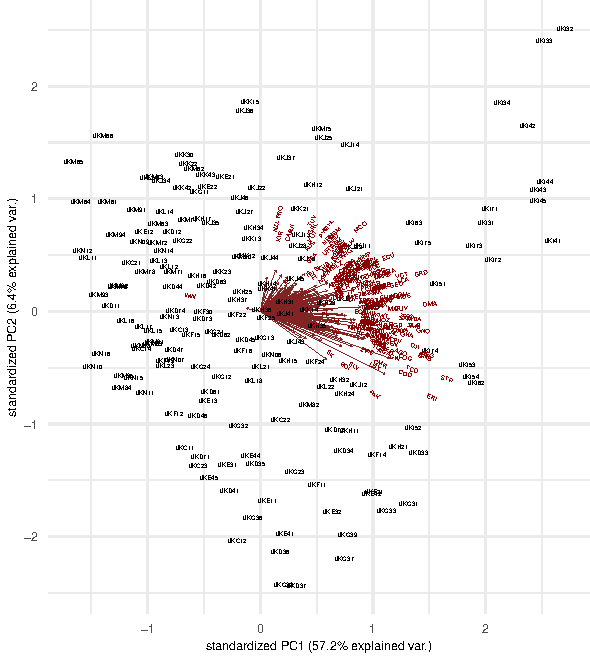
\includegraphics[width=0.8\linewidth]{SCI-and-Leave-Voting_files/figure-latex/biplot-1} 

}

\caption{Biplot of country-level SCI scores by UK NUTs area}\label{fig:biplot}
\end{figure}

Finally, EU-27 country-level SCI scores are merged using a population
weighted average to give each NUTS-3 region of the UK an SCI score for
the EU-27. This statistic is plotted in Figure \ref{fig:sci_map} along
with internal SCI. That is, the proportion of social connections within
the region which are fulfilled. The two indexes are compared in Figure
\ref{fig:scatter}.

\begin{figure}

{\centering 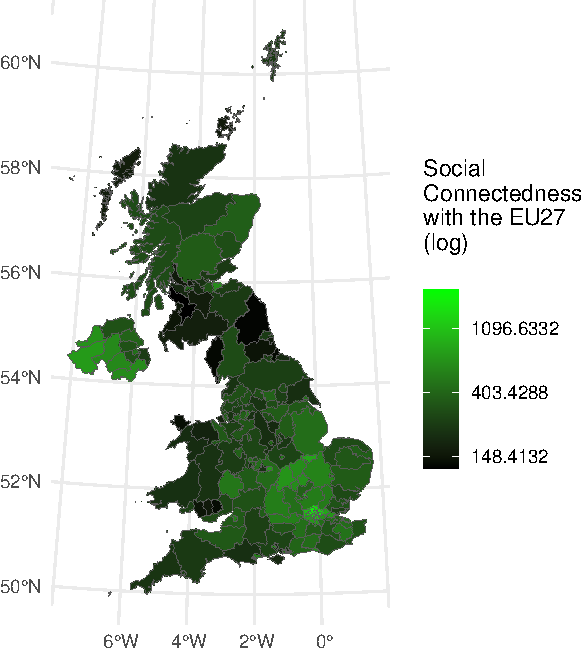
\includegraphics[width=0.49\linewidth]{SCI-and-Leave-Voting_files/figure-latex/eu members-1} 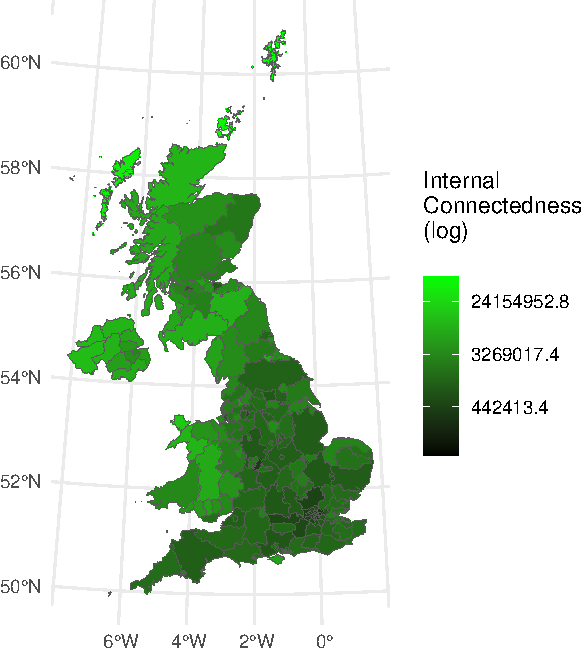
\includegraphics[width=0.49\linewidth]{SCI-and-Leave-Voting_files/figure-latex/eu members-2} 

}

\caption{\label{fig:sci_map}NUTS3 Regions by SCI with the EU-27 and interally}\label{fig:eu members}
\end{figure}

\begin{figure}

{\centering 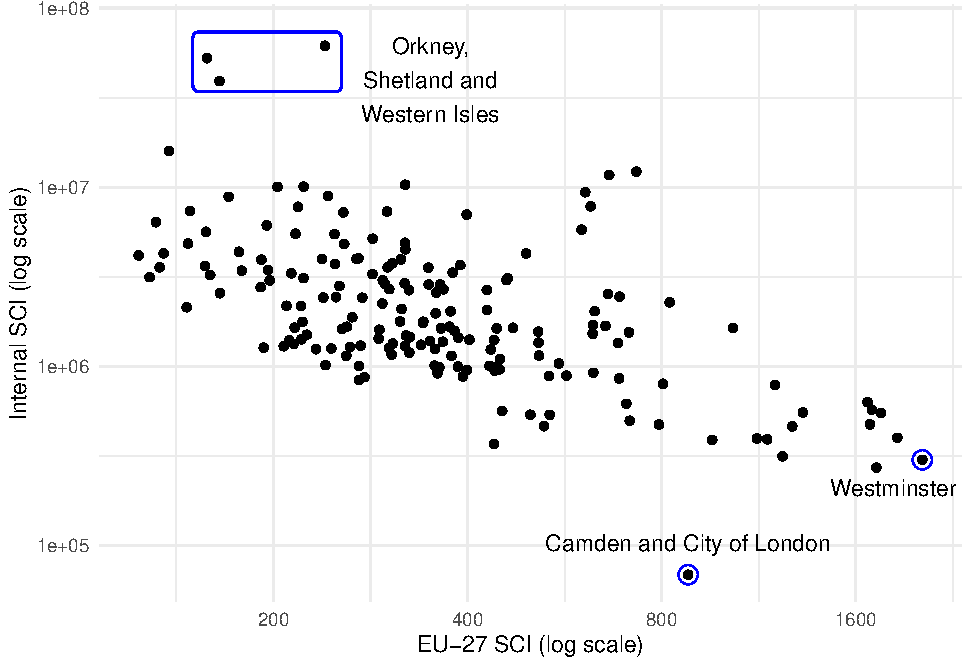
\includegraphics[width=0.8\linewidth]{SCI-and-Leave-Voting_files/figure-latex/scatter-1} 

}

\caption{\label{fig:scatter}Scatter Plot of Internal and EU-27 SCI Scores}\label{fig:scatter}
\end{figure}

\hypertarget{british-election-study}{%
\subsection{British Election Study}\label{british-election-study}}

The second main source of data is the British Election Study (BES)
(Fieldhouse and Eijk 2021). The BES is a large-scale survey of public
opinion, with data available at the level of individual respondents.
There are wide ranging questions including demographic variables, policy
preferences and past votes. BES is conducted using online surveys and a
random sample weighted to be representative of the population of Great
Britain. Wave 9, which includes the most relevant data for this study,
was conducted between 24th June 2016 and 4th July 2016 with 30,036
respondents.

To check the validity of BES, NUTS-level samples are compared to true EU
Referendum results Authority (2018). Figure \ref{fig:bes_validity} shows
how 76\% of NUTS regions have sample proportions within the 95\% margin
of error of true EU Referendum results for the sample size. This
suggests some sampling bias on top of statistical variance.

\begin{figure}

{\centering 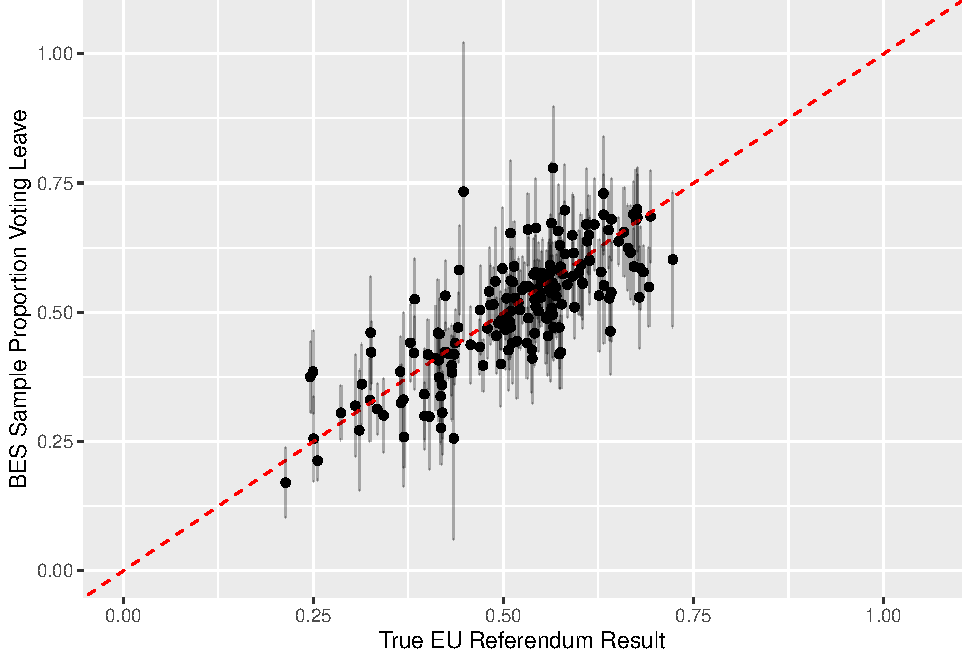
\includegraphics[width=0.8\linewidth]{SCI-and-Leave-Voting_files/figure-latex/bes_validity-1} 

}

\caption{Reported EU Referendum vote (BES) compared with true results at NUTs-level}\label{fig:bes_validity}
\end{figure}

\hypertarget{nuts-3-level-data}{%
\subsection{NUTS-3 Level Data}\label{nuts-3-level-data}}

Migration data is aggregated at the NUTS-level, using datasets provided
at local authority level by the Office for National Statistics Stickney
(2021b). This includes the proportion of residents born in the EU, the
rate of EU migration as a proportion of current population in 2016, and
change in rate of EU migration between 2011 and 2016. Finally, distances
between NUTS regions and the EU-27 are calculated. These distances are
measured from the centroid of each NUTS regions to the closest border of
the EU-27 (Figure \ref{fig:distances}).

\begin{figure}

{\centering 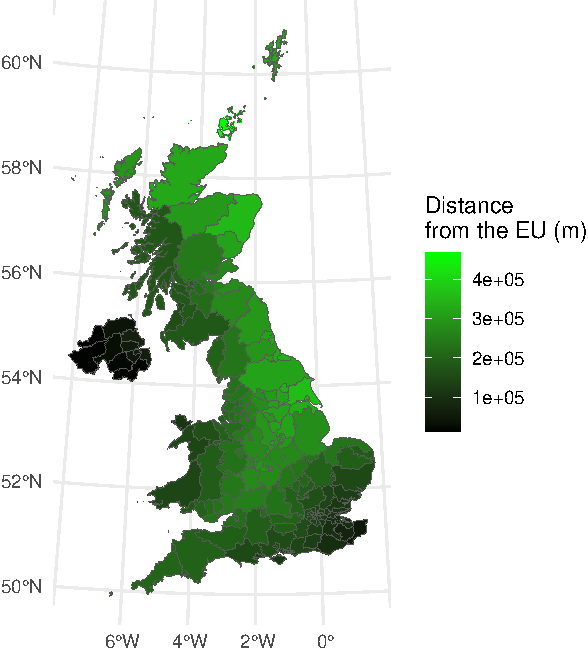
\includegraphics[width=0.5\linewidth]{SCI-and-Leave-Voting_files/figure-latex/distances-1} 

}

\caption{Distance to EU-27}\label{fig:distances}
\end{figure}

\hypertarget{methods}{%
\section{Methods}\label{methods}}

The primary method used is multilevel logistic regression (Gelman, Hill,
and Hill 2007). The dependent variable is self-reported vote to leave
the EU, of all those who voted in the 2016 Referendum, weighted using
BES weights. A multilevel model better represents the hierarchical
nature of survey data, with respondents nested within geographic or
demographic groups. In each case, respondents are drawn from broader
populations and the effect of these group-memberships is drawn from a
distribution of possible effects. In practice, this is useful because it
allows for partial pooling of the intercept and variance of each group,
leading to more accurate estimates including more robust standard errors
for fixed effects. In this study, we are most interested in the effect
of migration and social connections, so most other variables are
included as random effects.

\hypertarget{results}{%
\section{Results}\label{results}}

The first results to consider are of two correlation tests, between SCI
scores and the proportion of people born in the EU-27 (\textbf{H1}) and
between SCI scores and the proportion of people who voted to leave the
EU (\textbf{H4}) at NUTS level. In both cases, there is a significant
correlation, leading us to accept the hypotheses. The correlation
between SCI and EU-born population is particularly high (0.899) while
the correlation between SCI and leave-voting is less pronounced but
significant (-0.463).

\begin{table}[!htbp] \centering 
  \caption{Correlation Tests} 
  \label{table:cor} 
\begin{tabular}{@{\extracolsep{5pt}}lcc} 
\\[-1.8ex]\hline 
\hline \\[-1.8ex] 
\\[-1.8ex] & \multicolumn{2}{c}{Pearson's Product-Moment Correlation} \\ 
\\[-1.8ex] & \multicolumn{2}{c}{EU-27 Social Connectedness Index} \\ 
  & &  \\ 
\\[-1.8ex] & Percentage Born in EU & Leave Vote Percentage \\ 
\hline \\[-1.8ex] 
  & &  \\ 
 Estimate & 0.899$^{***}$ & -0.463$^{***}$ \\ 
  & &  \\ 
 Degrees of Freedom & 165 & 166 \\ 
 T-Statistic & 26.421 & -6.739 \\
 95\% Confidence Interval & [0.866, 0.925] & [-0.575, -0.336] \\
  & &  \\ 
\hline 
\hline \\[-1.8ex] 
\textit{Note:}  & \multicolumn{2}{r}{$.$ p$<$0.1; $^{*}$p$<$0.05; $^{**}$p$<$0.01; $^{***}$p$<$0.001} \\ 
\end{tabular} 
\end{table}

To consider \textbf{H2}, \textbf{H3} and \textbf{H5}, the results of
multilevel logistic regression is presented in Table
\ref{table:regression}.

In line with \textbf{H2} and \textbf{H3}, the rate of EU migration has a
negative effect on the likelihood of voting to leave the EU, while a
change in rate has a positive effect. However, these effects are not
significant in models 5 or 6, so there is insufficient evidence to
accept the hypotheses. In addition, rather than the expected negative
relationship between SCI and voting to leave (\textbf{H5}), there is a
small positive effect, which is not significant. This is the case across
all six models. Again, there is insufficient evidence to accept the
hypothesis. Perhaps the most interesting finding is that in both models
3 and 6, the internal SCI of a region has a significant positive effect.

\begin{table}[!htbp] \centering 
  \caption{Logistic Regression Models} 
  \label{table:regression} 
\begin{tabular}{@{\extracolsep{5pt}}lcccccc} 
\\[-1.8ex]\hline 
\hline \\[-1.8ex] 
 & \multicolumn{6}{c}{\textit{Dependent variable:}} \\ 
\cline{2-7} 
\\[-1.8ex] & \multicolumn{6}{c}{Leave Vote} \\ 
\\[-1.8ex] & (1) & (2) & (3) & (4) & (5) & (6)\\ 
\hline \\[-1.8ex] 
 Age (Scaled 0-1) & 1.789$^{***}$ & 1.156$^{***}$ & 1.146$^{***}$ & 1.150$^{***}$ & 1.150$^{***}$ & 1.145$^{***}$ \\ 
  & (0.059) & (0.081) & (0.081) & (0.081) & (0.081) & (0.074) \\ 
  & & & & & & \\ 
 Gender (Female = 1) & $-$0.087$^{**}$ & $-$0.149$^{***}$ & $-$0.150$^{***}$ & $-$0.149$^{***}$ & $-$0.149$^{***}$ & $-$0.149$^{***}$ \\ 
  & (0.029) & (0.036) & (0.036) & (0.036) & (0.036) & (0.033) \\ 
  & & & & & & \\ 
 EU Migration Inflow & $-$16.229$^{*}$ &  &  & $-$4.769 & $-$11.670 & $-$7.773 \\ 
 2016 (Per Capita) & (6.713) &  &  & (3.942) & (7.100) & (6.433) \\ 
  & & & & & & \\ 
 Inflow Change & 61.489$^{***}$ &  &  & 26.790$^{**}$ & 20.338$^{.}$ & 13.968 \\ 
 2011-2016 & (10.504) &  &  & (9.525) & (11.474) & (16.809) \\ 
  & & & & & & \\ 
 log( EU-27 SCI ) & 0.148 & 0.021 &  &  & 0.161 & 0.204$^{.}$ \\ 
  & (0.100) & (0.080) &  &  & (0.118) & (0.111) \\ 
  & & & & & & \\ 
 log( Internal SCI ) & 0.055 &  & 0.165$^{**}$ &  &  & 0.164$^{**}$ \\ 
  & (0.052) &  & (0.053) &  &  & (0.054) \\ 
  & & & & & & \\ 
 Distance from EU & 0.210 &  &  &  &  & 0.321 \\ 
 (Scaled 0-1) & (0.207) &  &  &  &  & (0.299) \\ 
  & & & & & & \\ 
 Constant & $-$2.247$^{*}$ & $-$1.008$^{.}$ & $-$3.230$^{***}$ & $-$0.835$^{*}$ & $-$1.713$^{*}$ & $-$4.478$^{***}$ \\ 
  & (1.085) & (0.580) & (0.833) & (0.341) & (0.730) & (1.130) \\ 
  & & & & & & \\ 
\hline \\[-1.8ex] 
\\[-1.8ex] & \multicolumn{6}{c}{Random Effects $\sigma^2$} \\ 
  & & & & & & \\
NUTS 3 & 0.106 & 0.092 & 0.077 & 0.087 & 0.087 & 0.074 \\
Gross Household Income & & 0.010 & 0.010 & 0.010 & 0.010 & 0.010 \\
Gross Personal Income & & 0.583 & 0.580 & 0.582 & 0.582 & 0.581 \\
Newspaper Read & & 0.009 & 0.009 & 0.009 & 0.009 & 0.009 \\
Ethnicity & & 0.223 & 0.224 & 0.224 & 0.225 & 0.226 \\
County of Birth & & 0.019 & 0.019 & 0.019 & 0.019 & 0.019 \\
UK Region & & 0.050 & 0.083 & 0.051 & 0.045 & 0.066 \\
Social Grade & & 0.079 & 0.079 & 0.079 & 0.079 & 0.079 \\
Education Level & & 0.188 & 0.189 & 0.187 & 0.187 & 0.187 \\
  & & & & & & \\ 
\hline \\[-1.8ex] 
Observations & 28,195 & 22,803 & 22,803 & 22,803 & 22,803 & 22,803 \\ 
Log Likelihood & $-$14,277 & $-$10,362 & $-$10,357 & $-$10,360 & $-$10,359 & $-$10,355 \\ 
Akaike Inf. Crit. & 28,571 & 20,750 & 20,741 & 20,748 & 20,748 & 20,743 \\ 
Bayesian Inf. Crit. & 28,645 & 20,855 & 20,845 & 20,860 & 20,869 & 20,880 \\ 
\hline 
\hline \\[-1.8ex] 
\textit{Note:}  & \multicolumn{6}{r}{$.$ p$<$0.1; $^{*}$p$<$0.05; $^{**}$p$<$0.01; $^{***}$p$<$0.001} \\ 
\end{tabular} 
\end{table}

\hypertarget{discussion-and-conclusion}{%
\section{Discussion and Conclusion}\label{discussion-and-conclusion}}

This study has not provided conclusive evidence of an effect of
transnational social connectedness on voting choices in the 2016 EU
Referendum. This may be due to the aggregation of SCI scores,
measurement error, confounding variables, or simply that the theorised
effect does not occur. One interesting result, which ought to be studied
further, is the significant positive relationship between voting to
leave the EU and internal SCI. Internal SCI shows connectedness within
regions, and tends to be highest in areas which are relatively isolated
(especially island regions). This may reflect suspicion of migration
and/or transnational institutions in tightly knit communities, or a
particular form of social transmission of euroscepticism. Internal SCI
is also likely to be closely correlated to areas with fewer links to
other areas of the UK, which may be related to narratives of regional
inequality and ``geography of discontent'' (Mccann and Ortega-Argilés
2021).

\hypertarget{r-packages}{%
\section*{R Packages}\label{r-packages}}
\addcontentsline{toc}{section}{R Packages}

\begin{itemize}
\tightlist
\item
  creditmodel (Fan 2022)
\item
  ggbiplot (Vu et al., n.d.)
\item
  ggforce (Pedersen 2021)
\item
  ggplot2 (Wickham 2016)
\item
  haven (Wickham and Miller 2022)
\item
  knitr (Xie 2021)
\item
  labelled (Larmarange et al., n.d.)
\item
  lme4 (Bates et al. 2015)
\item
  matrixStats (Bengtsson 2021)
\item
  readxl (Wickham and Bryan 2022)
\item
  rticles (Allaire et al. 2022)
\item
  sf (Pebesma 2018)
\item
  stargazer (Hlavac, n.d.)
\item
  stringr (Wickham 2019)
\item
  tidyverse (Wickham et al. 2019)
\end{itemize}

\hypertarget{bibliography}{%
\section*{Bibliography}\label{bibliography}}
\addcontentsline{toc}{section}{Bibliography}

\hypertarget{refs}{}
\begin{CSLReferences}{1}{0}
\leavevmode\vadjust pre{\hypertarget{ref-rticles}{}}%
Allaire, JJ, Yihui Xie, Christophe Dervieux, R Foundation, Hadley
Wickham, Journal of Statistical Software, Ramnath Vaidyanathan, et al.
2022. \emph{Rticles: Article Formats for r Markdown}.
\url{https://CRAN.R-project.org/package=rticles}.

\leavevmode\vadjust pre{\hypertarget{ref-results}{}}%
Authority, Greater London. 2018. {``EU Referendum Results.''} Dataset.
\url{https://data.gov.uk/dataset/be2f2aec-11d8-4bfe-9800-649e5b8ec044/eu-referendum-results}.

\leavevmode\vadjust pre{\hypertarget{ref-bailey2020}{}}%
Bailey, Michael, Drew Johnston, Theresa Kuchler, Dominic Russel, Bogdan
State, and Johannes Stroebel. 2020. {``The Determinants of Social
Connectedness in Europe.''} Book Section. In \emph{Lecture Notes in
Computer Science}, 1--14. Springer International Publishing.
\url{https://doi.org/10.1007/978-3-030-60975-7_1}.

\leavevmode\vadjust pre{\hypertarget{ref-sci}{}}%
Bailey, T. Kuchler, R. Cao, and A. Wong. 2018. {``Social Connectedness:
Measurements, Determinants, and Effects.''} Journal Article.
\emph{Journal of Economic Perspectives} 32 (3): 259--80.
\url{https://dataforgood.facebook.com/}.

\leavevmode\vadjust pre{\hypertarget{ref-lme4}{}}%
Bates, Douglas, Martin Mächler, Ben Bolker, and Steve Walker. 2015.
{``Fitting Linear Mixed-Effects Models Using {lme4}.''} \emph{Journal of
Statistical Software} 67 (1): 1--48.
\url{https://doi.org/10.18637/jss.v067.i01}.

\leavevmode\vadjust pre{\hypertarget{ref-matrixStats}{}}%
Bengtsson, Henrik. 2021. \emph{matrixStats: Functions That Apply to Rows
and Columns of Matrices (and to Vectors)}.
\url{https://CRAN.R-project.org/package=matrixStats}.

\leavevmode\vadjust pre{\hypertarget{ref-bettencourt2007}{}}%
Bettencourt, L. M., J. Lobo, D. Helbing, C. Kuhnert, and G. B. West.
2007. {``Growth, Innovation, Scaling, and the Pace of Life in Cities.''}
Journal Article. \emph{Proceedings of the National Academy of Sciences
of the United States of America} 104 (17): 7301--6.

\leavevmode\vadjust pre{\hypertarget{ref-enos2017}{}}%
Enos, Ryan D. 2017. {``The Space Between Us.''} Electronic Book.
Cambridge University Press.
\url{http://public.ebookcentral.proquest.com/choice/publicfullrecord.aspx?p=5212975}.

\leavevmode\vadjust pre{\hypertarget{ref-eurostat}{}}%
eurostat. 2021. {``Population Change - Demographic Balance and Crude
Rates at Regional Level (NUTS 3).''} Dataset. eurostat.

\leavevmode\vadjust pre{\hypertarget{ref-creditmodel}{}}%
Fan, Dongping. 2022. \emph{Creditmodel: Toolkit for Credit Modeling,
Analysis and Visualization}.
\url{https://CRAN.R-project.org/package=creditmodel}.

\leavevmode\vadjust pre{\hypertarget{ref-bes}{}}%
Fieldhouse, J. Green, E., and C. van der Eijk. 2021. {``British Election
Study Internet Panel Waves 1-21.''} Dataset.

\leavevmode\vadjust pre{\hypertarget{ref-gelmanhill2007}{}}%
Gelman, Andrew, Jennifer Hill, and Jennifer Hill. 2007. \emph{Data
Analysis Using Regression and Multilevel/Hierarchical Models}. Book.
Analytical Methods for Social Research. Cambridge ; Cambridge University
Press.
\url{http://catdir.loc.gov/catdir/enhancements/fy0668/2006040566-t.html\%0Ahttp://bvbr.bib-bvb.de:8991/F?func=service\&doc_library=BVB01\&doc_number=015428351\&line_number=0001\&func_code=DB_RECORDS\&service_type=MEDIA\%0Ahttp://bvbr.bib-bvb.de:8991/F?func=service\&doc_library=BVB01\&local_base=BVB01\&doc_number=015428351\&line_number=0001\&func_code=DB_RECORDS\&service_type=MEDIA\%0Ahttp://www.gbv.de/dms/ilmenau/toc/527420107.PDF\%0Ahttp://catdir.loc.gov/catdir/enhancements/fy0733/2006040566-b.html\%0Ahttp://catdir.loc.gov/catdir/enhancements/fy0668/2006040566-d.html}.

\leavevmode\vadjust pre{\hypertarget{ref-gadm}{}}%
Global Administrative Areas, Database of. 2022. {``GADM Maps and
Data.''} Web Page. \url{https://gadm.org/}.

\leavevmode\vadjust pre{\hypertarget{ref-goodwin2017}{}}%
Goodwin, Matthew, and Caitlin Milazzo. 2017. {``Taking Back Control?
Investigating the Role of Immigration in the 2016 Vote for Brexit.''}
Journal Article. \emph{The British Journal of Politics and International
Relations} 19 (3): 450--64.
\url{https://doi.org/10.1177/1369148117710799}.

\leavevmode\vadjust pre{\hypertarget{ref-stargazer}{}}%
Hlavac, Marek. n.d. {``Stargazer: Well-Formatted Regression and Summary
Statistics Tables. R Package Version 5.2.3.''} Computer Program.
\href{https://CRAN.R-project.org/package=stargazer\%20}{https://CRAN.R-project.org/package=stargazer}.

\leavevmode\vadjust pre{\hypertarget{ref-huckfeldt1987}{}}%
Huckfeldt, Robert, and John Sprague. 1987. {``Networks in Context: The
Social Flow of Political Information.''} \emph{American Political
Science Review} 81 (4): 1197--1216.
\url{https://doi.org/10.2307/1962585}.

\leavevmode\vadjust pre{\hypertarget{ref-labelled}{}}%
Larmarange, Joseph, Daniel Ludecke, Hadley Wickham, Michal Bojanowski,
and Francois Briatte. n.d. {``Labelled.''} Computer Program.
\url{https://larmarange.github.io/labelled/}.

\leavevmode\vadjust pre{\hypertarget{ref-lee2017}{}}%
Lee, Francis L. F., Paul S. N. Lee, Clement Yk So, Louis Leung, and
Michael Cheming Chan. 2017. {``Conditional Impact of Facebook as an
Information Source on Political Opinions: The Case of Political Reform
in Hong Kong.''} Journal Article. \emph{Asian Journal of Political
Science} 25 (3): 365--82.
\url{https://doi.org/10.1080/02185377.2017.1352523}.

\leavevmode\vadjust pre{\hypertarget{ref-mccann2021}{}}%
Mccann, Philip, and Raquel Ortega-Argilés. 2021. {``The UK {`Geography
of Discontent'}: Narratives, Brexit and Inter-Regional {`Levelling
up'}.''} Journal Article. \emph{Cambridge Journal of Regions, Economy
and Society} 14 (3): 545--64.
\url{https://doi.org/10.1093/cjres/rsab017}.

\leavevmode\vadjust pre{\hypertarget{ref-nurmuhammad2016}{}}%
Nurmuhammad, Rizwangul, Heather A. Horst, Evangelia Papoutsaki, and
Giles Dodson. 2016. {``Uyghur Transnational Identity on Facebook: On the
Development of a Young Diaspora.''} Journal Article. \emph{Identities}
23 (4): 485--99. \url{https://doi.org/10.1080/1070289x.2015.1024126}.

\leavevmode\vadjust pre{\hypertarget{ref-belfast_telegraph}{}}%
Peake, Gordon. 2014. {``Hard-Working, Respectful and Warm... We Could
Learn from Our Timorese Guests.''} Newspaper Article.
\url{https://www.belfasttelegraph.co.uk/opinion/columnists/hard-working-respectful-and-warm-we-could-learn-from-our-timorese-guests-30377313.html}.

\leavevmode\vadjust pre{\hypertarget{ref-sf}{}}%
Pebesma, Edzer. 2018. {``{Simple Features for R: Standardized Support
for Spatial Vector Data}.''} \emph{{The R Journal}} 10 (1): 439--46.
\url{https://doi.org/10.32614/RJ-2018-009}.

\leavevmode\vadjust pre{\hypertarget{ref-ggforce}{}}%
Pedersen, Thomas Lin. 2021. \emph{Ggforce: Accelerating 'Ggplot2'}.
\url{https://CRAN.R-project.org/package=ggforce}.

\leavevmode\vadjust pre{\hypertarget{ref-ons_migration}{}}%
Stickney, Chris. 2021a. {``Local Area Migration Indicators, UK.''}
Dataset.
\url{https://www.ons.gov.uk/peoplepopulationandcommunity/populationandmigration/migrationwithintheuk/datasets/localareamigrationindicatorsunitedkingdom}.

\leavevmode\vadjust pre{\hypertarget{ref-ons_cob}{}}%
---------. 2021b. {``Population of the UK by Country of Birth and
Nationality.''} Dataset.
\url{https://www.ons.gov.uk/peoplepopulationandcommunity/populationandmigration/internationalmigration/datasets/populationoftheunitedkingdombycountryofbirthandnationality}.

\leavevmode\vadjust pre{\hypertarget{ref-ggbiplot}{}}%
Vu, Vince, Ben Marwick, Jim Hester, and Max Held. n.d. {``Ggbiplot.''}
Computer Program.
\url{https://github.com/vqv/ggbiplot/tree/experimental}.

\leavevmode\vadjust pre{\hypertarget{ref-ggplot2}{}}%
Wickham, Hadley. 2016. \emph{Ggplot2: Elegant Graphics for Data
Analysis}. Springer-Verlag New York.
\url{https://ggplot2.tidyverse.org}.

\leavevmode\vadjust pre{\hypertarget{ref-stringr}{}}%
---------. 2019. \emph{Stringr: Simple, Consistent Wrappers for Common
String Operations}. \url{https://CRAN.R-project.org/package=stringr}.

\leavevmode\vadjust pre{\hypertarget{ref-tidyverse}{}}%
Wickham, Hadley, Mara Averick, Jennifer Bryan, Winston Chang, Lucy
D'Agostino McGowan, Romain François, Garrett Grolemund, et al. 2019.
{``Welcome to the Tidyverse.''} \emph{Journal of Open Source Software} 4
(43): 1686. \url{https://doi.org/10.21105/joss.01686}.

\leavevmode\vadjust pre{\hypertarget{ref-readxl}{}}%
Wickham, Hadley, and Jennifer Bryan. 2022. \emph{Readxl: Read Excel
Files}.

\leavevmode\vadjust pre{\hypertarget{ref-haven}{}}%
Wickham, Hadley, and Evan Miller. 2022. \emph{Haven: Import and Export
'SPSS', 'Stata' and 'SAS' Files}.

\leavevmode\vadjust pre{\hypertarget{ref-knitr}{}}%
Xie, Yihui. 2021. \emph{Knitr: A General-Purpose Package for Dynamic
Report Generation in r.}

\end{CSLReferences}

\bibliographystyle{unsrt}
\bibliography{references.bib}


\end{document}
